\section{Updating the networking protocol}\label{sec:update-network-protocol}
During implementation of the networking protocol outlined in \autoref{sec:sprint3-uppaal}, problems related to the implementation of acknowledgements in the UDP based connection for game critical data were encountered.
Section \ref{sec:sprint3-uppaal} defines the way the protocol was envisioned to work based on the choice made in \autoref{sec:sprint1-networking}, where UDP sockets were selected as the type to be used for this project.
\\
With the inherent unreliability of UDP it would be necessary to implement an acknowledgment from clients that they had received crucial data relating to the setup of the game, as defined in \autoref{sec:sprint3-uppaal}.
During the implementation of this, issues were encountered when sending the acknowledgment packet from the client to the host.
\\\\
As the sockets should make use of multicasting, as defined in \autoref{sec:sprint1-udptransmission}, our theory was that the clients should just be able to send packets to the same multicast group, and have the host receive that packet, with a type that specified that the packet was an acknowledgment that could be either positive or negative, structured in the same way as described in \autoref{subsec:data-format}.
However, the host had issues receiving the packets, where the packet would be sent to the multicast IP, but never received by the host.
\\
This prompted a discussion regarding how to remedy this issue, as a new approach seemed necessary.
Three main alternatives were considered:
\begin{itemize}
    \item Split the networking into two distinct phases - setup and in-game data
    \item Expand the packets being sent to include the crucial data on all packets sent
    \item Introduce a TCP element to make use of its reliability for game critical data
\end{itemize}

\subsubsection{Splitting networking into two distinct phases}
This approach aims to create a clear delineation between the crucial data that requires acknowledgment from clients and the data for which acknowledgments are unnecessary.
This was roughly the original approach, as shown on \autoref{fig:uppaal-host-1}, which illustrates how the host would wait in a setup state until acknowledgments had been received from all clients, and then the game would start.
\\
This presents issues in terms of the multicast grouping, in which the host was unable to read packets sent through the group.
This could be remedied by having a separate multicast group in which clients could send acknowledgments.
While the host was sending out the information, a client could check if it had received the correct information, and if not, send out a negative acknowledgment for a while before timing out, to attempt to receive the information again.
\\
Eventually all the clients would be sending positive acknowledgments.
\\\\
However, a limitation exists with this approach: when scoring a goal, it is crucial that the goal zones are moved.
This change of goal position would take place during the in-game phase, and receiving the information about the location of the new goal zone is crucial, such that all players know where to score.
As such, the phase split loses some of its purpose, as an acknowledgment would need to be sent from clients during the playing phase.

\subsubsection{Expanding packets}
In addition to the data defined in \autoref{app:network}, crucial data could be appended to all packets sent while the game is running.
This would mean that whenever any packet was received, it would include the required information, and no acknowledgment would be necessary as the clients normally will receive some packets if they are continuously sent.
This would have the detriment of increasing the size of each individual packet.
While the packets are currently not large enough to where this is likely to cause a problem, creating minimal packets is still a worthwhile goal in order to increase the speed of transmission and decoding.

\subsubsection{Introducing TCP}
On top of the currently described UDP approach to sending packets to ensure recent data is used for positioning while the game is played, a TCP socket connection between the host and clients could be implemented.
As described in \autoref{sec:sprint1-networking}, TCP includes reliability.
This reliability ensures that every packet sent will be received by the client, through built-in acknowledgments and re-transmissions.
This would remove the need for clients sending UDP acknowledgments for game crucial data, and also make the implementation of a sliding window as described in \autoref{sec:sliding-window} for UDP unnecessary.
Because of the reliability, and needing established connections, TCP packets could potentially be slower to transmit.
This would be the case if the TCP connection had to re-transmit a packet.
Re-transmitting a packet involves waiting for a timeout, which incurs the larger overhead in comparison to UDP.
As one of the focuses for the project is creating a networking solution capable of continuously updating positional data at a rate that makes the in-game positioning feel like real-time, this is not an ideal solution for transmitting the data when the game is being played.
\begin{table}[h!]
    \begin{tabular}{|l|l|l|l|}
        \hline
            & Plus                                                                                                            & Minus                                                                                                                         & Interesting                                                                                                                                                             \\ \hline
        TCP & \begin{tabular}[c]{@{}l@{}}Reliable\\ Built-in acknowledgements\\ Two way communication\end{tabular}            & \begin{tabular}[c]{@{}l@{}}Slower than UDP\\ More overhead because\\  of reliability and\\ two way communication\end{tabular} & \begin{tabular}[c]{@{}l@{}}For critical packets that concern \\ the state of the game TCP ensures \\ that all players receive \\ the update.\end{tabular}      \\ \hline
        UDP & \begin{tabular}[c]{@{}l@{}}Faster than TCP\\ Less overhead because it is a \\ one way communication\end{tabular} & \begin{tabular}[c]{@{}l@{}}Not reliable\\ No built-in \\ acknowledgements\end{tabular}                                      & \begin{tabular}[c]{@{}l@{}}Because UDP does not ensure that \\ the clients have received the \\ correct packets it can send \\ updates faster than TCP.\end{tabular} \\ \hline
    \end{tabular}
    \caption{PMI analysis of TCP and UDP}
    \label{Tab:PMI-TCP-UDP}
\end{table}
We performed a PMI (Plus Minus Interesting) analysis, as taught in the Software Innovation course, on both protocols to outline the strengths and weaknesses of TCP and UDP which can be seen in \autoref{Tab:PMI-TCP-UDP}.
As can be seen on the table, both approaches have specific use cases where they are useful, and in our case we have use cases for both TCP and UDP.
As such, a combination is proposed - TCP for crucial data, and UDP for positional data.
The issue described above relating to goal zones can also be remedied through a combination.
Rather than send location for the new goal zones while the game was being played and waiting for an acknowledgment, this data could be sent on the TCP connection as well.

\subsubsection{Final choice of updating}
Based on the three alternatives to remedy the issues encountered, introducing a separate TCP connection between the hosts and the clients to handle crucial data that requires acknowledgments seems like the ideal choice.
It avoids the confusion inherent in the unreliability of UDP requiring manual handling of acknowledgments, and avoids communication back and forth while allowing fast update times for positional data through the UDP connection.
Facilitating these changes would entail a slight change in the deployment diagram shown in \autoref{fig:sprint2-deployment}.
An association would have to be added between the host and client nodes indicating the new TCP connection, which is shown on \autoref{fig:sprint4-deployment}.
The dependency between the host and client application has also been updated to indicate that the client depends on both configuration and positional data.
\begin{figure}[H]
    \centering
    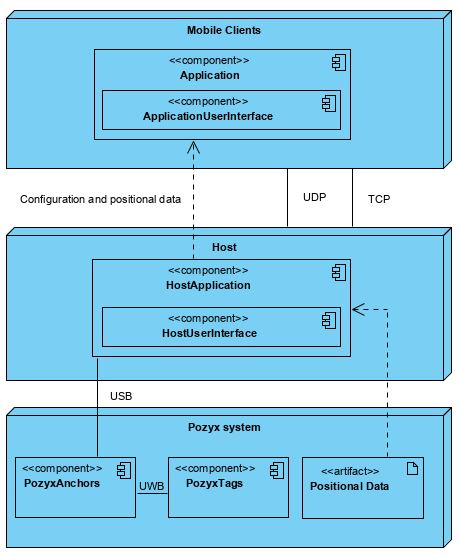
\includegraphics[width=0.6\linewidth]{sprint4/deployment-sprint4.JPG}
    \caption{A slightly revised deployment diagram for the system.}
    \label{fig:sprint4-deployment}
\end{figure}
\noindent
